In this section we first sketch the software architecture of SDN networks, and then describe some examples
of errors observed in production software-defined networks.

\subsection{SDN Architecture}

SDN networks are managed by software running on a set of network-attached servers called ``controllers''. This software is comprised of three distinct layers, as
depicted in Figure \ref{fig:basicarch}. The two lower layers are part of the SDN platform, and the highest layer is the control application. We now describe the functions of each layer.

\noindent{\bf Control Application:} This component specifies the desired
high-level behavior of the network. We terms these behavioral specifications ``policies''. It is the job of the SDN platform to implement these high-level policy-specifications by configuring the forwarding tables of the physical switches, and the platform does so in two steps, each implemented in a separate layer.

\noindent{\bf Physical View:} The lowest level of SDN software maintains a graph data-structure known as
the `physical view', that has a one-to-one correspondence with the physical
network. When informed from above about a new policy,
synchronization logic in this layer generates a set of configuration changes and sends them to the
corresponding network devices. Conversely, when a state change
occurs in the network (links going down, new ports installed, etc.), this layer notifies the layer above of the change.

\noindent{\bf Logical View:} The middle layer in the SDN software architecture is sometimes called the virtualization layer because it translates the (possibly complicated) physical view into a simpler logical view. A common pattern (and the one we focus on here) is to represent an entire
datacenter network as a single logical
switch~\cite{Casado:2010:VNF:1921151.1921162}. This allows operators
to specify routing, access control, and QoS policies by configuring a single forwarding
device. Thus, network policies (emanating from the control application) can be
expressed as a set of flow entries $<header, actions>$ where possible actions
includes primitives such as forward out a particular port, drop, or encrypt, and the possible ports include all edge ports (either connecting to external networks, or to hosts). Such a specification would dictate how any packet entering the network should be handled: i.e., what outgoing edge port it should be forwarded to, and perhaps what middlebox services it should be subject to along the way.   
In addition to providing a simplified network view, the virtualization layer
can support multi-tenancy by providing each tenant with their own logical
network to specify policies over. The platform then multiplexes the policies onto the same physical network.
\scott{do we use the F(view) anywhere? Let's take it out of the diagram and
remove it from the text.} \colin{agreed. (waiting for laptop to dry out)}

\eat{
, and isolates control applications from the specifics
of the underlying network. Ideally, \colin{Be clear that we aren't tied to
f(view). This technique applies to any network policy specification model} each application is reduced to a
state-less, side-effect free function~\cite{keynote}:
\begin{align*}
f(\text{\it view}) \rightarrow \text{\it configuration}
\end{align*}
}

The logical view greatly simplifies the job of specifying policies. But SDN
does not eliminate complexity; it merely moves it into the platform, which
must transform these high-level policy specifications into the appropriate
configuration of each physical device. Because modern datacenter networks are
large (easily reaching thousands of switches and a hundred thousand hosts),
the SDN platform must be replicated across many servers.
Onix~\cite{onix}, for example,
partitions a graph of the network state across either an eventually-consistent
DHT or a transactional database, allowing control applications to make their own
tradeoffs in choosing consistency models, degree of
fault tolerance, and other properties.

The large scale of these networks also means that error events such as link
failures or software crashes are common.
For example, Microsoft reports 36M 
error events over one year across 8 datacenters,
which implies 8.5 error events per minute per
datacenter~\cite{Greenberg:2009:VSF:1592568.1592576}. Thus, the SDN control platform is a complicated distributed system operating in a highly dynamic environment, making troubleshooting both hard and necessary.

\begin{figure}[t]
    %\hspace{-10pt}
    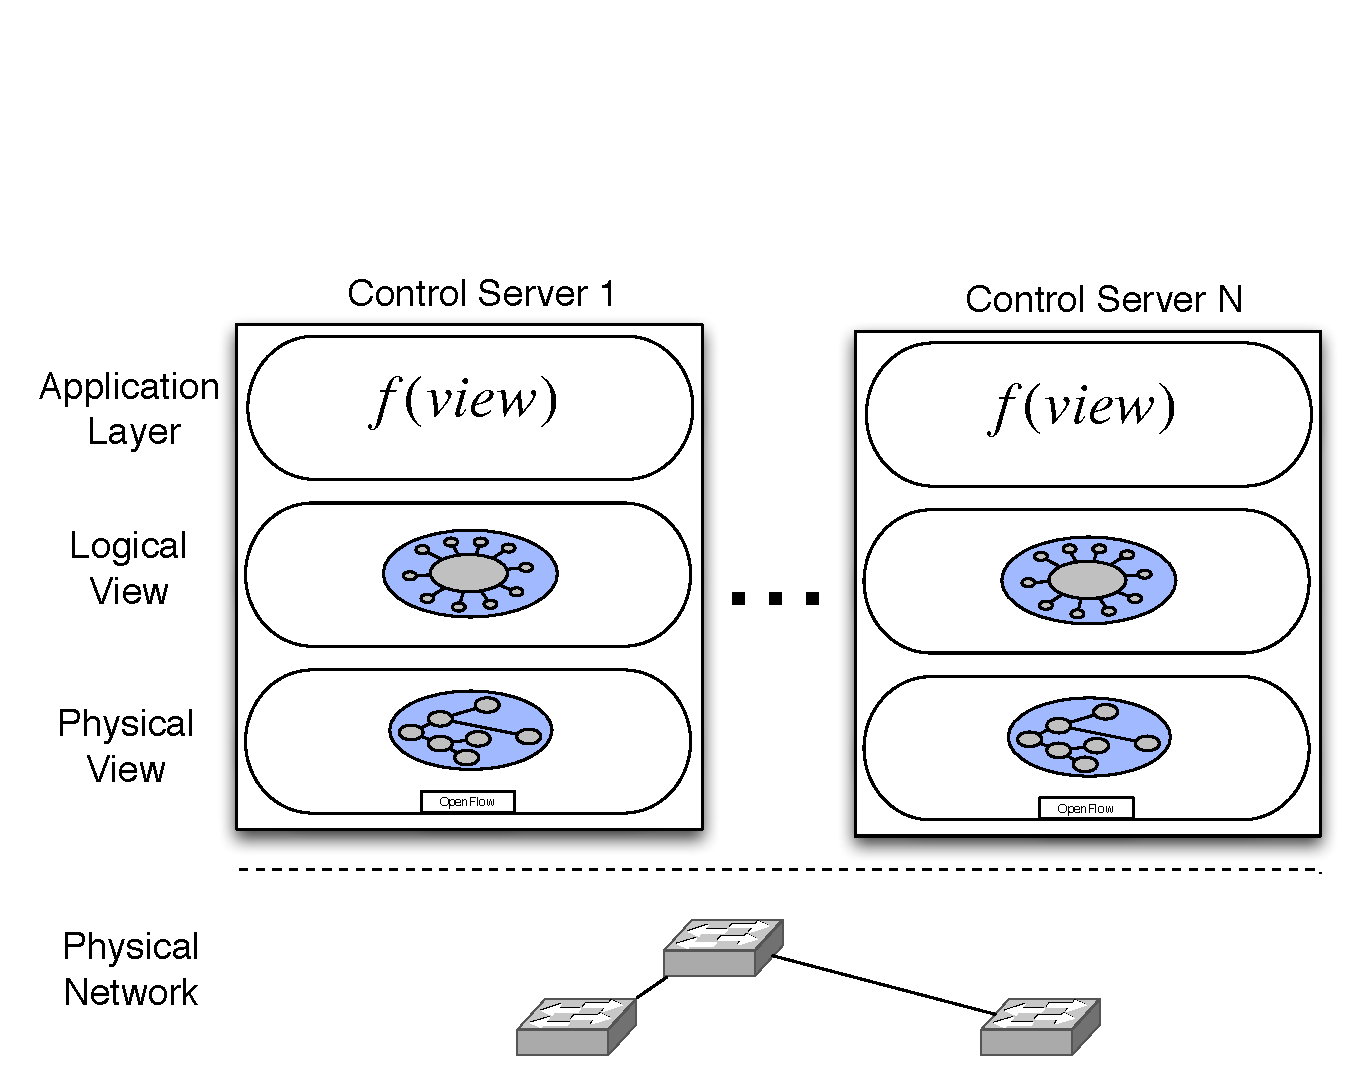
\includegraphics[width=3.25in]{../diagrams/architecture/SDN_Stack.pdf}
    \caption[]{\label{fig:basicarch} The SDN Software Architecture } 
\end{figure}

SDN control applications may express proactively or reactively.
Proactive applications pre-compute forwarding tables for the entire network,
and only push down updates periodically to react to link failures, changes in
traffic mix, \etc. In contrast, reactive control applications forward all new flows to
control servers. After a control decision is made, a flow entry is installed
in the ingress switch, and the packet is forwarded along.
Production SDN deployments are commonly proactive, primarily due to the large
scale of datacenter networks and the current capabilities of forwarding hardware.
We focus on proactive controllers for the remainder of this paper,
although our troubleshooting mechanisms are also applicable to reactive
applications.

\subsection{Platform Failure Modes}

\projectname{} is designed to troubleshoot the SDN platform; here we discuss a few examples of platform failures. 
As described above, modern SDN platforms differ from
`first-generation' controllers such as NOX~\cite{nox} in two dimensions: 
they extend vertically by providing a virtualization layer on top of
which control logic resides, and they extend horizontally by
distributing state across multiple control servers. Platform errors arise from both of
these extensions.

\noindent{\bf Virtualization}. Virtualization errors often result from a
mismatch between the logical
view and the state of the physical network. Consider that an entire datacenter
network (up to 10,000 switches) may be abstracted into a single logical switch. Especially in the
presence of hardware failures, the mapping between the logical switch and the
physical topology is highly complex. In a multi-tenant environment, the mapping is often
many-to-many~\cite{Casado:2010:VNF:1921151.1921162}; each tenant specifies
policies on their own logical switch, while the platform multiplexes each
slice over the same physical network. If the logical address
spaces are not disjoint, or a change in the physical network causes the paths
to temporarily overlap, breaches of tenant isolation or failure to properly
install configuration changes may occur,

\noindent{\bf Controller Coordination}. Coordination between controllers
entails the same classes of error
conditions that arise in general distributed systems: inconsistent reads and
writes, race conditions over message arrivals, and unintended consequences of failover
logic are common. As an example, suppose a controller fails, and all the
switches under its purview are adopted by a new control server. If the new parent
neglects to properly query the switches for their current state, or reads
stale control information from the data store, it may inadvertently install
conflicting flow entries in the network. Errors may also result 
from non-disjoint partitioning
schemes between controllers, or incorrect delegation of control for different
portions of the network. 
High churn in the network topology due to VM migration and
hardware failures exacerbate these issues.

%All of these errors may manifest as dataplane forwarding problems, such as
%loops, blackholes, partitions, broadcast storms. Or breaches of isolation in
%multi-tenant environments. Or just failure to push routing or ACL or QoS
%policys to switches. Also Route flapping. Or (preventable) congestion.
